\documentclass[UTF8,a4paper,11pt]{article}

\usepackage{ctex} 
\usepackage{fancyhdr}
\usepackage{multicol} 
\usepackage{lastpage} 
\usepackage{geometry} 
\usepackage{hyperref}
\usepackage{titlesec} 
\usepackage{mathrsfs}
\usepackage{graphicx}
\usepackage{epstopdf}
\usepackage{ulem}
\usepackage{amsmath}
\usepackage[subfigure,AllowH]{graphfig} 

\geometry{left=3cm,right=3cm,top=2.5cm,bottom=2.5cm}
\renewcommand{\baselinestretch}{1.5}
\everymath{\displaystyle}


\title{\huge\heiti《电磁场与电磁波基础》笔记}
\author{AlwaysLoveMisaka}
\date{\today}

\begin{document}
\maketitle
\thispagestyle{empty}
\clearpage

\tableofcontents
\setcounter{page}{1}
\pagenumbering{Roman}
\clearpage


\setcounter{page}{1}
\pagenumbering{arabic}
\section{前言}
这篇文章是我写的一篇关于《电磁场与电磁波基础》(电子工业出版社)的复习手册。我打算利用这个手册梳理一下电磁场与电磁波的重点知识。同志们在使用这个手册的时候,最好要结合课本,我也会在文中提及课本第三版的内容。

因为这个复习手册是我边学边写的,所以可能会有一些错误。另外,此手册也不能作为考点参考,因为我也不知道考试到底考啥。

这个手册是在Github上免费提供的,以后也会同步到CSDN上,如果同志们觉得这个好用,可以给我的内容点一个赞。如果有同志发现我写的内容有问题,可以加我qq——876563962,我会及时回复。本人Github主页:\url{https://github.com/AlwaysLoveMisaka},CSDN主页:\url{https://blog.csdn.net/Communism1848?spm=1000.2115.3001.5343}。

这个手册可以写出来,我首先要感谢的是魏勤老师,她既是教材的编者之一,也是我《电磁场与电磁波基础》这门课授课老师。我认为这种情况对于我个人是非常难得的,没有她对教材的深入讲解,我估计写不出来什么东西。我还要感谢我的父母,他们给我的大学生活提供了经济支持。

另外,我还要感谢小鸟游六花(如图1),虽然她是一个虚拟的人物,但却是我真实的\sout{老婆}精神支柱。在22年7月的时候,我因为一些事情的影响,被确诊轻度焦虑抑郁障碍。是小鸟游六花陪着我度过了那一段最难熬的日子,我一直很感激她。
\begin{figure}[htbp]
\centering
\includegraphics[scale=0.3]{p1.png}
\caption{小鸟游六花}
\end{figure}

\section{矢量分析与场论}
\subsection{矢量的表示与运算}
在三维直角坐标系中,矢量$\overrightarrow{A}$表示为:
\begin{equation}
\overrightarrow{A}=A_x\overrightarrow{e_x}+A_y\overrightarrow{e_y}+A_z\overrightarrow{e_z}
\end{equation}

式中,矢量$\overrightarrow{A}$的模为$\left| \overrightarrow{A} \right|=\sqrt{A_x^2+A_y^2+A_z^2}$,而$\overrightarrow{e_x}$、$\overrightarrow{e_y}$、$\overrightarrow{e_z}$分别为直角坐标系$x$、$y$、$z$轴方向上的矢量。

矢量相加满足交换律与结合律。

两矢量$\overrightarrow{A}$与$\overrightarrow{B}$的\textbf{标积}记为$\overrightarrow{A}\cdot\overrightarrow{B}$,结果为一个标量。
\begin{equation}
\overrightarrow{A}\cdot\overrightarrow{B}=\left| \overrightarrow{A} \right| \left| \overrightarrow{B} \right| \cos\theta_{AB}=A_xB_x+A_yB_y+A_zB_z
\end{equation}

式中,$\theta_{AB}$为两矢量夹角,两矢量的标积满足交换律和分配律。

两矢量$\overrightarrow{A}$与$\overrightarrow{B}$的\textbf{矢积}记为$\overrightarrow{A}\times\overrightarrow{B}$。两矢量进行矢积后的结果仍是个矢量,满足分配律,其大小等于两矢量的模之积再乘以两矢量夹角的正弦,矢积的方向符合右手定则,如图2。
\begin{figure}[htbp]
\centering
\includegraphics[scale=0.1]{p2.jpg}
\caption{右手定则}
\end{figure}

矢积与两矢量的直角坐标分量的关系为:
\begin{equation}
\overrightarrow{A}\times\overrightarrow{B}=\overrightarrow{e_x}(A_yB_z-A_zB_y)+\overrightarrow{e_y}(A_zB_x-A_xB_z)+\overrightarrow{e_z}(A_xB_y-A_yB_x)
\end{equation}

上式也可以写成行列式形式:
\begin{equation}
\overrightarrow{A}\times\overrightarrow{B}=\begin{vmatrix}
\overrightarrow{e_x} & \overrightarrow{e_y} &\overrightarrow{e_z} \\
A_x & A_y & A_z \\
B_x & B_y & B_z \\
\end{vmatrix}
\end{equation}

矢积有如下性质:
\begin{equation}
\overrightarrow{A}\times\overrightarrow{B}=-\overrightarrow{B}\times\overrightarrow{A}
\end{equation}
\begin{equation}
\overrightarrow{A}\cdot(\overrightarrow{B}\times\overrightarrow{C})=\overrightarrow{B}\cdot(\overrightarrow{C}\times\overrightarrow{A})=\overrightarrow{C}\cdot(\overrightarrow{A}\times\overrightarrow{B})
\end{equation}
\begin{equation}
\overrightarrow{A}\times(\overrightarrow{B}\times\overrightarrow{C})=(\overrightarrow{A}\cdot\overrightarrow{C})\overrightarrow{B}-(\overrightarrow{A}\cdot\overrightarrow{B})\overrightarrow{C}
\end{equation}

\subsection{坐标系}
在直角坐标系中,空间任意一点的位置都可以用三个独立的变量$x$、$y$、$z$表示,如图3。
\begin{figure}[htbp]
\centering
\includegraphics[scale=0.2]{p3.png}
\caption{直角坐标系}
\end{figure}

记$M(x,y,z)$是空间内一点,且$\overrightarrow{A}=\overrightarrow{OM}$,当$M$在空间中做微小移动到达$M'$时,$\overrightarrow{MM'}$就是矢量$\overrightarrow{A}$沿该方向的\textbf{微分线元},可表示为:
\begin{equation}
\overrightarrow{MM'}={\rm d}\overrightarrow{l}={\rm d}x\overrightarrow{e_x}+{\rm d}y\overrightarrow{e_y}+{\rm d}z\overrightarrow{e_z}
\end{equation}

直角坐标系中还存在一种很特殊的矢量,称为\textbf{面积元},可表示为:
\begin{equation}
\begin{cases}
{\rm d}\overrightarrow{S_x}={\rm d}y{\rm d}z\overrightarrow{e_x} \\
{\rm d}\overrightarrow{S_y}={\rm d}x{\rm d}z\overrightarrow{e_y} \\
{\rm d}\overrightarrow{S_z}={\rm d}x{\rm d}y\overrightarrow{e_z} \\
\end{cases}
\end{equation}

对于闭合曲面,面元的方向为该曲面的外法线方向。对于非闭合曲面,面元的方向要在曲面边界的环绕方向选定后,根据右手螺旋定则来确定。相似的,体积元可以表示为${\rm d}V={\rm d}x{\rm d}y{\rm d}z$。

空间任意一点的位置也可以用三个独立的变量$r$、$\phi$、$z$表示,这是圆柱坐标系的三个变量,如图4。
\begin{figure}[htbp]
\centering
\includegraphics[scale=0.2]{p4.png}
\caption{圆柱坐标系}
\end{figure}

圆柱坐标系变量与直角坐标系变量的关系是:
\begin{equation}
\begin{cases}
x=r\cos\phi \\
y=r\sin\phi \\
z=z \\
\end{cases}
\end{equation}
\begin{equation}
\begin{cases}
r=\sqrt{x^2+y^2} \\
\phi={\rm arctan}\frac{y}{x} \\
z=z \\
\end{cases}
\end{equation}

同理,空间任意一点也可以用$R$、$\phi$、$\theta$来表示,这是球坐标系,如图5。
\begin{figure}[htbp]
\centering
\includegraphics[scale=0.2]{p5.jpg}
\caption{球坐标系}
\end{figure}

球坐标系变量与直角坐标系变量的关系是:
\begin{equation}
\begin{cases}
x=R\sin\theta\cos\phi \\
y=R\sin\theta\sin\phi \\
z=R\cos\theta \\
\end{cases}
\end{equation}
\begin{equation}
\begin{cases}
R=\sqrt{x^2+y^2+z^2} \\
\phi={\rm arctan}\frac{y}{x} \\
\theta={\rm arctan}\frac{\sqrt{x^2+y^2}}{z} \\
\end{cases}
\end{equation}

球坐标系变量与圆柱坐标系变量的关系是:
\begin{equation}
\begin{cases}
r=R\sin\theta \\
\phi=\phi \\
z=R\cos\theta \\
\end{cases}
\end{equation}
\begin{equation}
\begin{cases}
R=\sqrt{r^2+z^2} \\
\phi=\phi \\
\theta={\rm arctan}\frac{r}{z} \\
\end{cases}
\end{equation}

圆柱坐标系和球坐标系的微分线元、面积元的表示可参见教材p7。

\subsection{矢量函数的通量与散度}
在研究电场、磁场时,可借助一组场线(矢量线)来形象地表示矢量场的空间分布,如描述电场的电力线、描述磁场的磁力线等。矢量场中每一点都有唯一的一条矢量线通过,线的疏密表示该点矢量场的强弱。

\textbf{通量}可以认为是矢量$\overrightarrow{A}$穿过曲面$S$的矢量线总数。矢量线也叫通量线,穿出为正,穿入为负。矢量场$\overrightarrow{A}$也可称为通量面密度矢量。通量$\Phi$的定义式为:
\begin{equation}
\Phi=\int_S {\overrightarrow{A}}\cdot \,{\rm d}\overrightarrow{S}
\end{equation}

矢量场$\overrightarrow{A}$在空间中一点\textbf{散度}的定义式为:
\begin{equation}
{\rm div}\overrightarrow{A}=\lim_{\Delta V \to 0} \frac{\oint {\overrightarrow{A}}\cdot \,{\rm d}\overrightarrow{S}}{\Delta V}
\end{equation}

${\rm div}\overrightarrow{A}$表示在场中任意一点处通量对体积的变化率, 也可看成是在该点处单位体积通过的通量,它表示了场中各点的场与通量源的关系。散度的运算满足分配律,通量与散度都是标量。

通过一系列证明可知:
\begin{equation}
{\rm div}\overrightarrow{A}=\frac{\partial A_x}{\partial x}+\frac{\partial A_y}{\partial y}+\frac{\partial A_z}{\partial z}
\end{equation}

引入一个微分算子$\nabla$,称为哈密顿算子,即
\begin{equation}
\nabla=\overrightarrow{e_x}\frac{\partial}{\partial x}+\overrightarrow{e_y}\frac{\partial}{\partial y}+\overrightarrow{e_z}\frac{\partial}{\partial z}
\end{equation}

因此
\begin{equation}
{\rm div}\overrightarrow{A}=\nabla\cdot\overrightarrow{A}
\end{equation}

$\nabla$是一个很重要的微分算子,它有两重意义。首先,它具有矢量特性,而不是一个具体的矢量。其次,它是微分算符,它对跟随其后的函数进行微分,不论跟随其后的函数是矢量函数还是标量函数。

可以证明:
\begin{equation}
\int_V \nabla\cdot\overrightarrow{A} \,{\rm d}V=\oint_S {\overrightarrow{A}}\cdot \,{\rm d}\overrightarrow{S}
\end{equation}

此等式被称为高斯散度定理。

\subsection{矢量函数的环量与旋度}
在矢量场中,任取一闭合路径$l$,矢量函数$\overrightarrow{A}$,沿闭合路径$l$的积分
\begin{equation}
C=\oint_l {\overrightarrow{A}}\cdot \,{\rm d}\overrightarrow{l}
\end{equation}
称为矢量函数$\overrightarrow{A}$沿闭合曲线$l$的\textbf{环量}。

\textbf{旋度}和环量的关系与散度和通量的关系类似,但是有一点不同。即使把一个闭合曲线收缩至一个点,它还是有法线方向的,因此旋度的定义如下:
\begin{equation}
{\rm rot}\overrightarrow{A}=max(\lim_{\Delta S \to 0} \frac{\oint {\overrightarrow{A}}\cdot \,{\rm d}\overrightarrow{l}}{\Delta S})
\end{equation}

可以证明:
\begin{equation}
\begin{aligned}
{\rm rot}\overrightarrow{A}&=\overrightarrow{e_x}(\frac{\partial A_z}{\partial y}-\frac{\partial A_y}{\partial z})+\overrightarrow{e_y}(\frac{\partial A_x}{\partial z}-\frac{\partial A_z}{\partial x})+\overrightarrow{e_z}(\frac{\partial A_y}{\partial x}-\frac{\partial A_x}{\partial y}) \\
&=\nabla\times\overrightarrow{A}
\end{aligned}
\end{equation}

为了方便记忆,可以用行列式表示为:
\begin{equation}
\nabla\times\overrightarrow{A}=\begin{vmatrix}
\overrightarrow{e_x} & \overrightarrow{e_y} &\overrightarrow{e_z} \\
\frac{\partial}{\partial x} & \frac{\partial}{\partial y} & \frac{\partial}{\partial z} \\
A_x & A_y & A_z \\
\end{vmatrix}
\end{equation}

值得注意的是,虽然环量是标量,但是旋度是矢量,旋度的计算满足分配律。斯托克斯定理说明了环量与旋度之间的关系:
\begin{equation}
\int_S \nabla\times\overrightarrow{A} \,{\rm d}\overrightarrow{S}=\oint_l {\overrightarrow{A}}\cdot \,{\rm d}\overrightarrow{l}
\end{equation}

旋度还有一个重要性质:任何一个矢量的旋度的散度恒等于0。即
\begin{equation}
\nabla\cdot(\nabla\times\overrightarrow{A})=0
\end{equation}

\subsection{标量函数的梯度}
一个标量函数$u(x,y,z)$的\textbf{梯度}的定义式为:
\begin{equation}
{\rm grad}u=\overrightarrow{e_x}\frac{\partial u}{\partial x}+\overrightarrow{e_y}\frac{\partial u}{\partial y}+\overrightarrow{e_z}\frac{\partial u}{\partial z}=\nabla u
\end{equation}

由上式可以看出,一个标量场的梯度是一个矢量场。在电磁学理论中,电位场的梯度就是电场强度取负。梯度运算满足分配律。

梯度有如下性质:
\begin{equation}
\nabla\times\nabla u=0
\end{equation}
\begin{equation}
\nabla f(u)=f'(u)\nabla u
\end{equation}
\begin{equation}
\nabla\cdot\nabla u=\nabla^2u=\frac{\partial^2 u}{\partial x^2}+\frac{\partial^2 u}{\partial y^2}+\frac{\partial^2 u}{\partial z^2}
\end{equation}

$\nabla^2$被称为拉普拉斯算子,其在直角坐标系有
\begin{equation}
\nabla^2=\frac{\partial^2}{\partial x^2}+\frac{\partial^2}{\partial y^2}+\frac{\partial^2}{\partial z^2}
\end{equation}

对一个标量场进行拉普拉斯运算,结果也是一个标量场。

\subsection{亥姆霍兹定理}
前几节的知识可以说明:散度表示矢量场中各点的场与通量源的关系而旋度表示场中各点场与涡旋源的关系。因此,场的散度和旋度且给定,就意味着场的通量源和涡旋源就确定了。既然场总是由源所激发的,通量源和涡旋源的确定便意味着场已确定,因而可得出下述亥姆霍兹定理给出的结论:一个矢量场的散度和旋度说明了矢量场所具有的性质,而且可以证明:在有限区域$V$内的任一矢量场,由它的散度、旋度和边界条件(即限定区域$V$的闭合面$S$上矢量场的分布)唯一地确定。也就是说通过哈密顿算符我们可以确定一个场的散度和旋度,反过来,我们知道一个场的散度和旋度,也可以反过来唯一确定一个场。

通过亥姆霍兹定理,我们可以把场分为\textbf{无旋场}、\textbf{无源场}和\textbf{有源有旋场}。

如果一个场的每一点都有$\nabla\times\overrightarrow{F}=0$,那么这个场只有通量源,我们称矢量场$\overrightarrow{F}$为无旋场。对于任意一个无旋场,都存在一个标量函数$\phi$,使得
\begin{equation}
\overrightarrow{F}=-\nabla\phi
\end{equation}

函数$\phi$被称为无旋场$\overrightarrow{F}$的\textbf{标量位函数},此式说明可以在电场中引入电位函数来描述电场这个矢量。由斯托克斯定理可知:
\begin{equation}
\oint_C {\overrightarrow{F}}\cdot \,{\rm d}\overrightarrow{l}=0
\end{equation}

由上式可知,无旋场的曲线积分与路径无关,静电场和引力场都属于无旋场。

如果一个场的每一点都有$\nabla\cdot\overrightarrow{F}=0$,那么这个场只有涡旋源,我们称矢量场$\overrightarrow{F}$为无源场。对于任意一个无源场,都存在一个矢量函数$\overrightarrow{A}$,使得
\begin{equation}
\overrightarrow{F}=\nabla\times\overrightarrow{A}
\end{equation}

函数$\overrightarrow{A}$被称为无源场$\overrightarrow{F}$的\textbf{矢量位函数}。由高斯定理可知:
\begin{equation}
\oint_S {\overrightarrow{F}}\cdot \,{\rm d}\overrightarrow{S}=0
\end{equation}

由上式可知,无源场的闭曲面积分为0,磁场属于典型的无源场。

有源有旋场同时具有非零的散度和非零的旋度,时变电磁场和运云动电荷产生的电场就是此类,此时有:
\begin{equation}
\nabla\cdot\overrightarrow{F}=\rho
\end{equation}
\begin{equation}
\nabla\times\overrightarrow{F}=\overrightarrow{J}
\end{equation}

式中,$\rho$表示通量源,$\overrightarrow{J}$表示涡旋源。根据亥姆霍兹定理,一个普通矢量场 F可以分解为无旋部分$\overrightarrow{F_i}$(保守场)和无源部分$\overrightarrow{F_{\rho}}$(管形场),即
\begin{equation}
\overrightarrow{F}=\overrightarrow{F_i}+\overrightarrow{F_{\rho}}
\end{equation}

可以定义一个标量位函数$\phi$和一个矢量位函数$\overrightarrow{A}$,使得
\begin{equation}
\overrightarrow{F_i}=-\nabla\phi
\end{equation}
\begin{equation}
\overrightarrow{F_{\rho}}=\nabla\times\overrightarrow{A}
\end{equation}

因此,若矢量场F在无限空间中处处单值,且其导数连续有界,而源分布在有限区域中,则矢量场由其散度和旋度唯一地确定。并且,它可表示为一个标量函数的梯度和一个矢量函数的旋度之和。

\section{自由空间的电磁场}
\subsection{电场强度和电位}
由高中的知识可知,电荷之间存在作用力,力的大小和方向满足库仑定律:
\begin{equation}
\overrightarrow{F_E}=\frac{qq'}{4\pi\epsilon_0R^2}\overrightarrow{e_R}
\end{equation}

式中$\epsilon_0$称为\textbf{真空介电常数},其大小为$\epsilon_0=(1/36\pi)\times10^{-9}F/m$。假定电荷$q=1C$,于是电场力$\overrightarrow{F_E}$即为$q$对单位电荷的作用力,我们将这个特定大小的电场力称为\textbf{电场强度}$\overrightarrow{E}$。
\begin{equation}
\overrightarrow{E}=\frac{q'}{4\pi\epsilon_0R^2}\overrightarrow{e_R}
\end{equation}

如果电荷是沿以曲线连续分布的,且线电荷密度为$\rho_l$,则其在空间中产生的电场强度为:
\begin{equation}
\overrightarrow{E}=\frac{1}{4\pi\epsilon_0}\int_l{\frac{\rho_l{\rm d}l}{R^2}\overrightarrow{e_R}}
\end{equation}

同理。如果电荷沿一曲面连续分布或者在某空间体积连续分布,它们产生的电场强度为:
\begin{equation}
\overrightarrow{E}=\frac{1}{4\pi\epsilon_0}\int_S{\frac{\rho_S{\rm d}S}{R^2}\overrightarrow{e_R}}
\end{equation}
\begin{equation}
\overrightarrow{E}=\frac{1}{4\pi\epsilon_0}\int_V{\frac{\rho{\rm d}V}{R^2}\overrightarrow{e_R}}
\end{equation}

因为电场强度是一个无旋场,因此有
\begin{equation}
\overrightarrow{E}=-\nabla\phi
\end{equation}

$\phi$被称为\textbf{电位},是一个标量场。

\subsection{磁感应强度}
就像用电场强度描述电场一样,我们可以用\textbf{磁感应强度}$\overrightarrow{B}$描述磁场。假设电荷$q$以速度$\overrightarrow{v}$在磁场中运动,它所受到的磁场力可以表示为
\begin{equation}
\overrightarrow{F_B}=q\overrightarrow{v}\times\overrightarrow{B}
\end{equation}

\begin{figure}[htbp]
\centering
\includegraphics[scale=0.6]{p6.png}
\caption{毕奥-萨伐尔定律}
\end{figure}
高中物理学教材告诉我们,电流周围可以产生磁场,毕奥-萨伐尔定律(如图6)揭示了电流激发磁场的定量关系:
\begin{equation}
\overrightarrow{B}=\frac{\mu_0}{4\pi}\oint_l\frac{I{\rm d}l\times\overrightarrow{e_R}}{R^2}
\end{equation}
式中$\mu_0$称为\textbf{真空磁导率},其大小为$4\pi\times10^{-7}H/m$。

同理,如果电流分布在一个连续曲面或者一体积内,上述定律可改写为
\begin{equation}
\overrightarrow{B}=\frac{\mu_0}{4\pi}\int_S\frac{\overrightarrow{J_S}\times\overrightarrow{e_R}}{R^2}{\rm d}S
\end{equation}
\begin{equation}
\overrightarrow{B}=\frac{\mu_0}{4\pi}\int_V\frac{\overrightarrow{J}\times\overrightarrow{e_R}}{R^2}{\rm d}V
\end{equation}

可以证明:
\begin{equation}
\nabla\cdot\overrightarrow{B}=0
\end{equation}

由上式可以看出,磁力线总是连续的,它不会在闭合曲面内积累或中断。

\subsection{全电流定律}
上一节我们知道了如何使用电流计算其周围的磁场,相同的,我们也可以通过磁感应强度计算电流。安培环路定律如下:
\begin{equation}
\oint_l\overrightarrow{B}\cdot{\rm d}\overrightarrow{l}=\mu_0I
\end{equation}

\begin{figure}[htbp]
\centering
\includegraphics[scale=0.3]{p7.jpg}
\caption{安培环路}
\end{figure}
式中环路必须环绕目标电流(如图7)。引入\textbf{磁场强度}$\overrightarrow{H}=\overrightarrow{B}/\mu_0$,则安培环路定律可改写为:
\begin{equation}
\oint_l\overrightarrow{H}\cdot{\rm d}\overrightarrow{l}=I
\end{equation}

在电磁场理论中,我们将电流分为三种不同的种类:传导电流、运流电流和位移电流。

传导电流是人们最为熟悉的一种电流,它是自由电荷在导电介质中作有规则运动而形成的。产生这种电流的根本原因是导电介质中存在电场的作用。因为传导电流满足欧姆定律,可以证明传导电流密度
\begin{equation}
\overrightarrow{J_c}=\sigma\overrightarrow{E}
\end{equation}

式中$\sigma$为\textbf{电导率}。假设$\rho$为电荷密度,可以得出一些传导电流的性质:
\begin{equation}
\nabla\cdot\overrightarrow{J_c}=-\int_V\frac{\partial\rho}{\partial t}{\rm d}V
\end{equation}

对上式应用高斯定理,可得:
\begin{equation}
\nabla\cdot\overrightarrow{J_c}=-\frac{\partial\rho}{\partial t}
\end{equation}

式(56)(57)被称为\textbf{电流连续性方程}。

电荷在无阻力空间,由于电场力作用或由于机械原因而产生规则运动时,将形成运流电流。空间上一点内,传导电流或运流电流一般不能共存。

由于回路中传导电流连续是安培环路定律成立的前提,但是在电流和磁场随时间变化时,传导电流可能不连续。因此麦克斯韦扩充了电流的概念:假设在电容器两极板之间,由于电场随时间的变化而在两极板之间存在位移电流,其数值等于流向极板的传导电流。

为了计算出位移电流,我们引入\textbf{电通量密度}$\overrightarrow{D}=\epsilon_0\overrightarrow{E}$,可以证明,位移电流密度
\begin{equation}
\overrightarrow{J_d}=\frac{\partial \overrightarrow{D}}{\partial t}
\end{equation}

引入位移电流的概念后,我们可以将安培环路定律推广到时变场情况。可以证明:
\begin{equation}
\oint_l\overrightarrow{H}\cdot{\rm d}\overrightarrow{l}=\int_S(\overrightarrow{J}+\frac{\partial \overrightarrow{D}}{\partial t})\cdot{\rm d}\overrightarrow{S}
\end{equation}

式中,$\overrightarrow{J}$是导体中的传导电流密度。上式表明,磁场不仅能有传导电流或运流电流产生,同时也能由变化的电流产生。对上式应用斯托克斯定理,可得
\begin{equation}
\nabla\times\overrightarrow{H}=\overrightarrow{J}+\frac{\partial \overrightarrow{D}}{\partial t}
\end{equation}

式(59)(60)被称为全电流定律,也被称为\textbf{麦克斯韦第一方程}。

\subsection{电磁感应定律}
\begin{figure}[htbp]
\centering
\includegraphics[scale=0.3]{p8.jpg}
\caption{法拉第电磁感应定律}
\end{figure}
高中物理告诉我们,变化的磁场可以激发感应电动势(如图8),感应电动势的定量表达为:
\begin{equation}
\epsilon_i=-\frac{{\rm d}\Phi_m}{{\rm d}t}
\end{equation}

通过我们之前学习的场论知识,我们可以将上式改写为:
\begin{equation}
\oint_l\overrightarrow{E}\cdot{\rm d}\overrightarrow{l}=\int_S-\frac{\partial\overrightarrow{B}}{\partial t}\cdot{\rm d}\overrightarrow{S}
\end{equation}

对上式应用斯托克斯定理,可得
\begin{equation}
\nabla\times\overrightarrow{E}=-\frac{\partial\overrightarrow{B}}{\partial t}
\end{equation}

式(62)(63)被称为\textbf{麦克斯韦第二方程}。

\subsection{高斯定律}
对式(52)应用高斯定理可以推出:
\begin{equation}
\oint_S\overrightarrow{B}\cdot{\rm d}\overrightarrow{S}=0
\end{equation}

式(52)(64)被称为\textbf{麦克斯韦第三方程},也被称为磁场的高斯定律。

电场也有属于自己的高斯定律:
\begin{equation}
\oint_S\overrightarrow{D}\cdot{\rm d}\overrightarrow{S}=Q
\end{equation}

对上式应用高斯定理,可得
\begin{equation}
\nabla\cdot\overrightarrow{D}=\rho
\end{equation}

式(65)(66)被称为\textbf{麦克斯韦第四方程}。
\begin{figure}[htbp]
\centering
\includegraphics[scale=2]{p9.png}
\caption{电场的高斯定律}
\end{figure}

电场的高斯定律可以让我们很轻松地计算出一些典型电场的场强,下面举几个例子。

(1)平面$xoy$均匀分布着面密度为$\rho_s$的电荷,求空间场强分布

我们可以构造一个垂直于$xoy$的柱体,取其上表面$S_0$(电场强度方向一定平行于$z$),因此
\begin{equation}
\begin{aligned}
DS_0&=\frac{S_0\rho_s}{2}\\
E&=\frac{\rho_s}{2\epsilon_0}
\notag
\end{aligned}
\end{equation}

(2)直线$z$均匀分布着线密度为$\rho_l$的电荷,求空间场强分布
我们可以构造一个以$z$为轴的柱体,取其测面(电场强度方向一定沿$r$方向),因此
\begin{equation}
\begin{aligned}
D2\pi rl_0&=\rho_ll_0\\
E&=\frac{\rho_l}{2\pi r\epsilon_0}
\notag
\end{aligned}
\end{equation}

\subsection{麦克斯韦方程组}
将前几节四个积分形式的麦克斯韦方程进行汇总,可得:
\begin{equation}
\begin{cases}
\oint_l\overrightarrow{H}\cdot{\rm d}\overrightarrow{l}=\int_S(\overrightarrow{J}+\frac{\partial \overrightarrow{D}}{\partial t})\cdot{\rm d}\overrightarrow{S}\\
\oint_l\overrightarrow{E}\cdot{\rm d}\overrightarrow{l}=\int_S-\frac{\partial\overrightarrow{B}}{\partial t}\cdot{\rm d}\overrightarrow{S}\\
\oint_S\overrightarrow{B}\cdot{\rm d}\overrightarrow{S}=0\\
\oint_S\overrightarrow{D}\cdot{\rm d}\overrightarrow{S}=Q\\
\end{cases}
\end{equation}
以及介质特性方程
\begin{equation}
\begin{cases}
\overrightarrow{B}=\mu_0\overrightarrow{H}\\
\overrightarrow{D}=\epsilon_0\overrightarrow{E}\\
\overrightarrow{J_c}=\sigma\overrightarrow{E}\\
\end{cases}
\end{equation}

以上即为麦克斯韦所总结的积分形式(包括三个介质特性方程)的电磁场方程组,又称为电磁场的完整方程组。第一和第二方程描述了电场与磁场相互依存,相互制约并且相互转化的关系。第三方程表明,磁场为无源场。第四方程表明,电场是有源场,即电场可以由点源电荷所激发。

将前几节四个微分形式的麦克斯韦方程进行汇总,可得:
\begin{equation}
\begin{cases}
\nabla\times\overrightarrow{H}=\overrightarrow{J}+\frac{\partial \overrightarrow{D}}{\partial t}\\
\nabla\times\overrightarrow{E}=-\frac{\partial\overrightarrow{B}}{\partial t}\\
\nabla\cdot\overrightarrow{B}=0\\
\nabla\cdot\overrightarrow{D}=\rho\\
\end{cases}
\end{equation}

以上即为麦克斯韦方程组的微分形式。第一方程强调了电场和磁场之间的内在联系,同时也指出了产生磁场的源是电流、移动电荷或者变化的电场。第二方程表明了随时间变化的磁场会产生电场。第三方程说明不存在“点磁荷”。第四方程说明电场的散度源是电荷。

\textbf{静态场}是指电磁场中源量和场量都不随时间变化的场,包括静电场、恒定电场和恒定磁场,是时变电磁场的特例。静电场是相对静止且不随时间变化的静电荷所产生的电场,恒定电场是在恒定电流产生的电场,这两者统一称为静态电场。分布不变的恒定电场所形成的恒定电流会导致恒定磁场的产生,恒定磁场又称为静态磁场。静态电场与静态磁场统称为静态电磁场,简称静态场。

静态场的麦克斯韦方程组积分形式
\begin{equation}
\begin{cases}
\oint_l\overrightarrow{H}\cdot{\rm d}\overrightarrow{l}=\int_S\overrightarrow{J}\cdot{\rm d}\overrightarrow{S}\\
\oint_l\overrightarrow{E}\cdot{\rm d}\overrightarrow{l}=0\\
\oint_S\overrightarrow{B}\cdot{\rm d}\overrightarrow{S}=0\\
\oint_S\overrightarrow{D}\cdot{\rm d}\overrightarrow{S}=Q\\
\end{cases}
\end{equation}

静态场的麦克斯韦方程组微分形式
\begin{equation}
\begin{cases}
\nabla\times\overrightarrow{H}=\overrightarrow{J}\\
\nabla\times\overrightarrow{E}=0\\
\nabla\cdot\overrightarrow{B}=0\\
\nabla\cdot\overrightarrow{D}=\rho\\
\end{cases}
\end{equation}

时变电磁场的一种最重要的类型是时间简谐场,简称\textbf{时谐场}。所谓时谐场,即激励源按照单一频率随时间作正弦变化时所激发的也随时间按照正弦变化的场。根据电路理论中的相量法,我们可以用相量来表示随正弦变化的场量。即
\begin{equation}
\begin{aligned}
E_x(x,y,z,t)&=E_{xm}(x,y,z)\cos(\omega t+\theta_x)\\
&=Re[E_{xm}(x,y,z)e^{j(\omega t+\theta_x)}]\\
&=Re[\dot{E}_{xm}(x,y,z)e^{j\omega t}]
\end{aligned}
\end{equation}

如果正弦函数$f(t)$以复指数形式表示,那么其导数就为$j\omega f(t)$。因此,微分算子$\frac{\partial}{\partial t}$可以用$j\omega$代替,得出复数形式的麦克斯韦方程组:
\begin{equation}
\begin{cases}
\oint_l\overrightarrow{H}\cdot{\rm d}\overrightarrow{l}=\int_S(\overrightarrow{J}+j\omega\overrightarrow{D})\cdot{\rm d}\overrightarrow{S}\\
\oint_l\overrightarrow{E}\cdot{\rm d}\overrightarrow{l}=\int_S-j\omega\overrightarrow{B}\cdot{\rm d}\overrightarrow{S}\\
\oint_S\overrightarrow{B}\cdot{\rm d}\overrightarrow{S}=0\\
\oint_S\overrightarrow{D}\cdot{\rm d}\overrightarrow{S}=Q\\
\end{cases}
\end{equation}

\begin{equation}
\begin{cases}
\nabla\times\overrightarrow{H}=\overrightarrow{J}+j\omega\overrightarrow{D}\\
\nabla\times\overrightarrow{E}=-j\omega\overrightarrow{B}\\
\nabla\cdot\overrightarrow{B}=0\\
\nabla\cdot\overrightarrow{D}=\rho\\
\end{cases}
\end{equation}

\subsection{坡印廷矢量}
\begin{figure}[htbp]
\centering
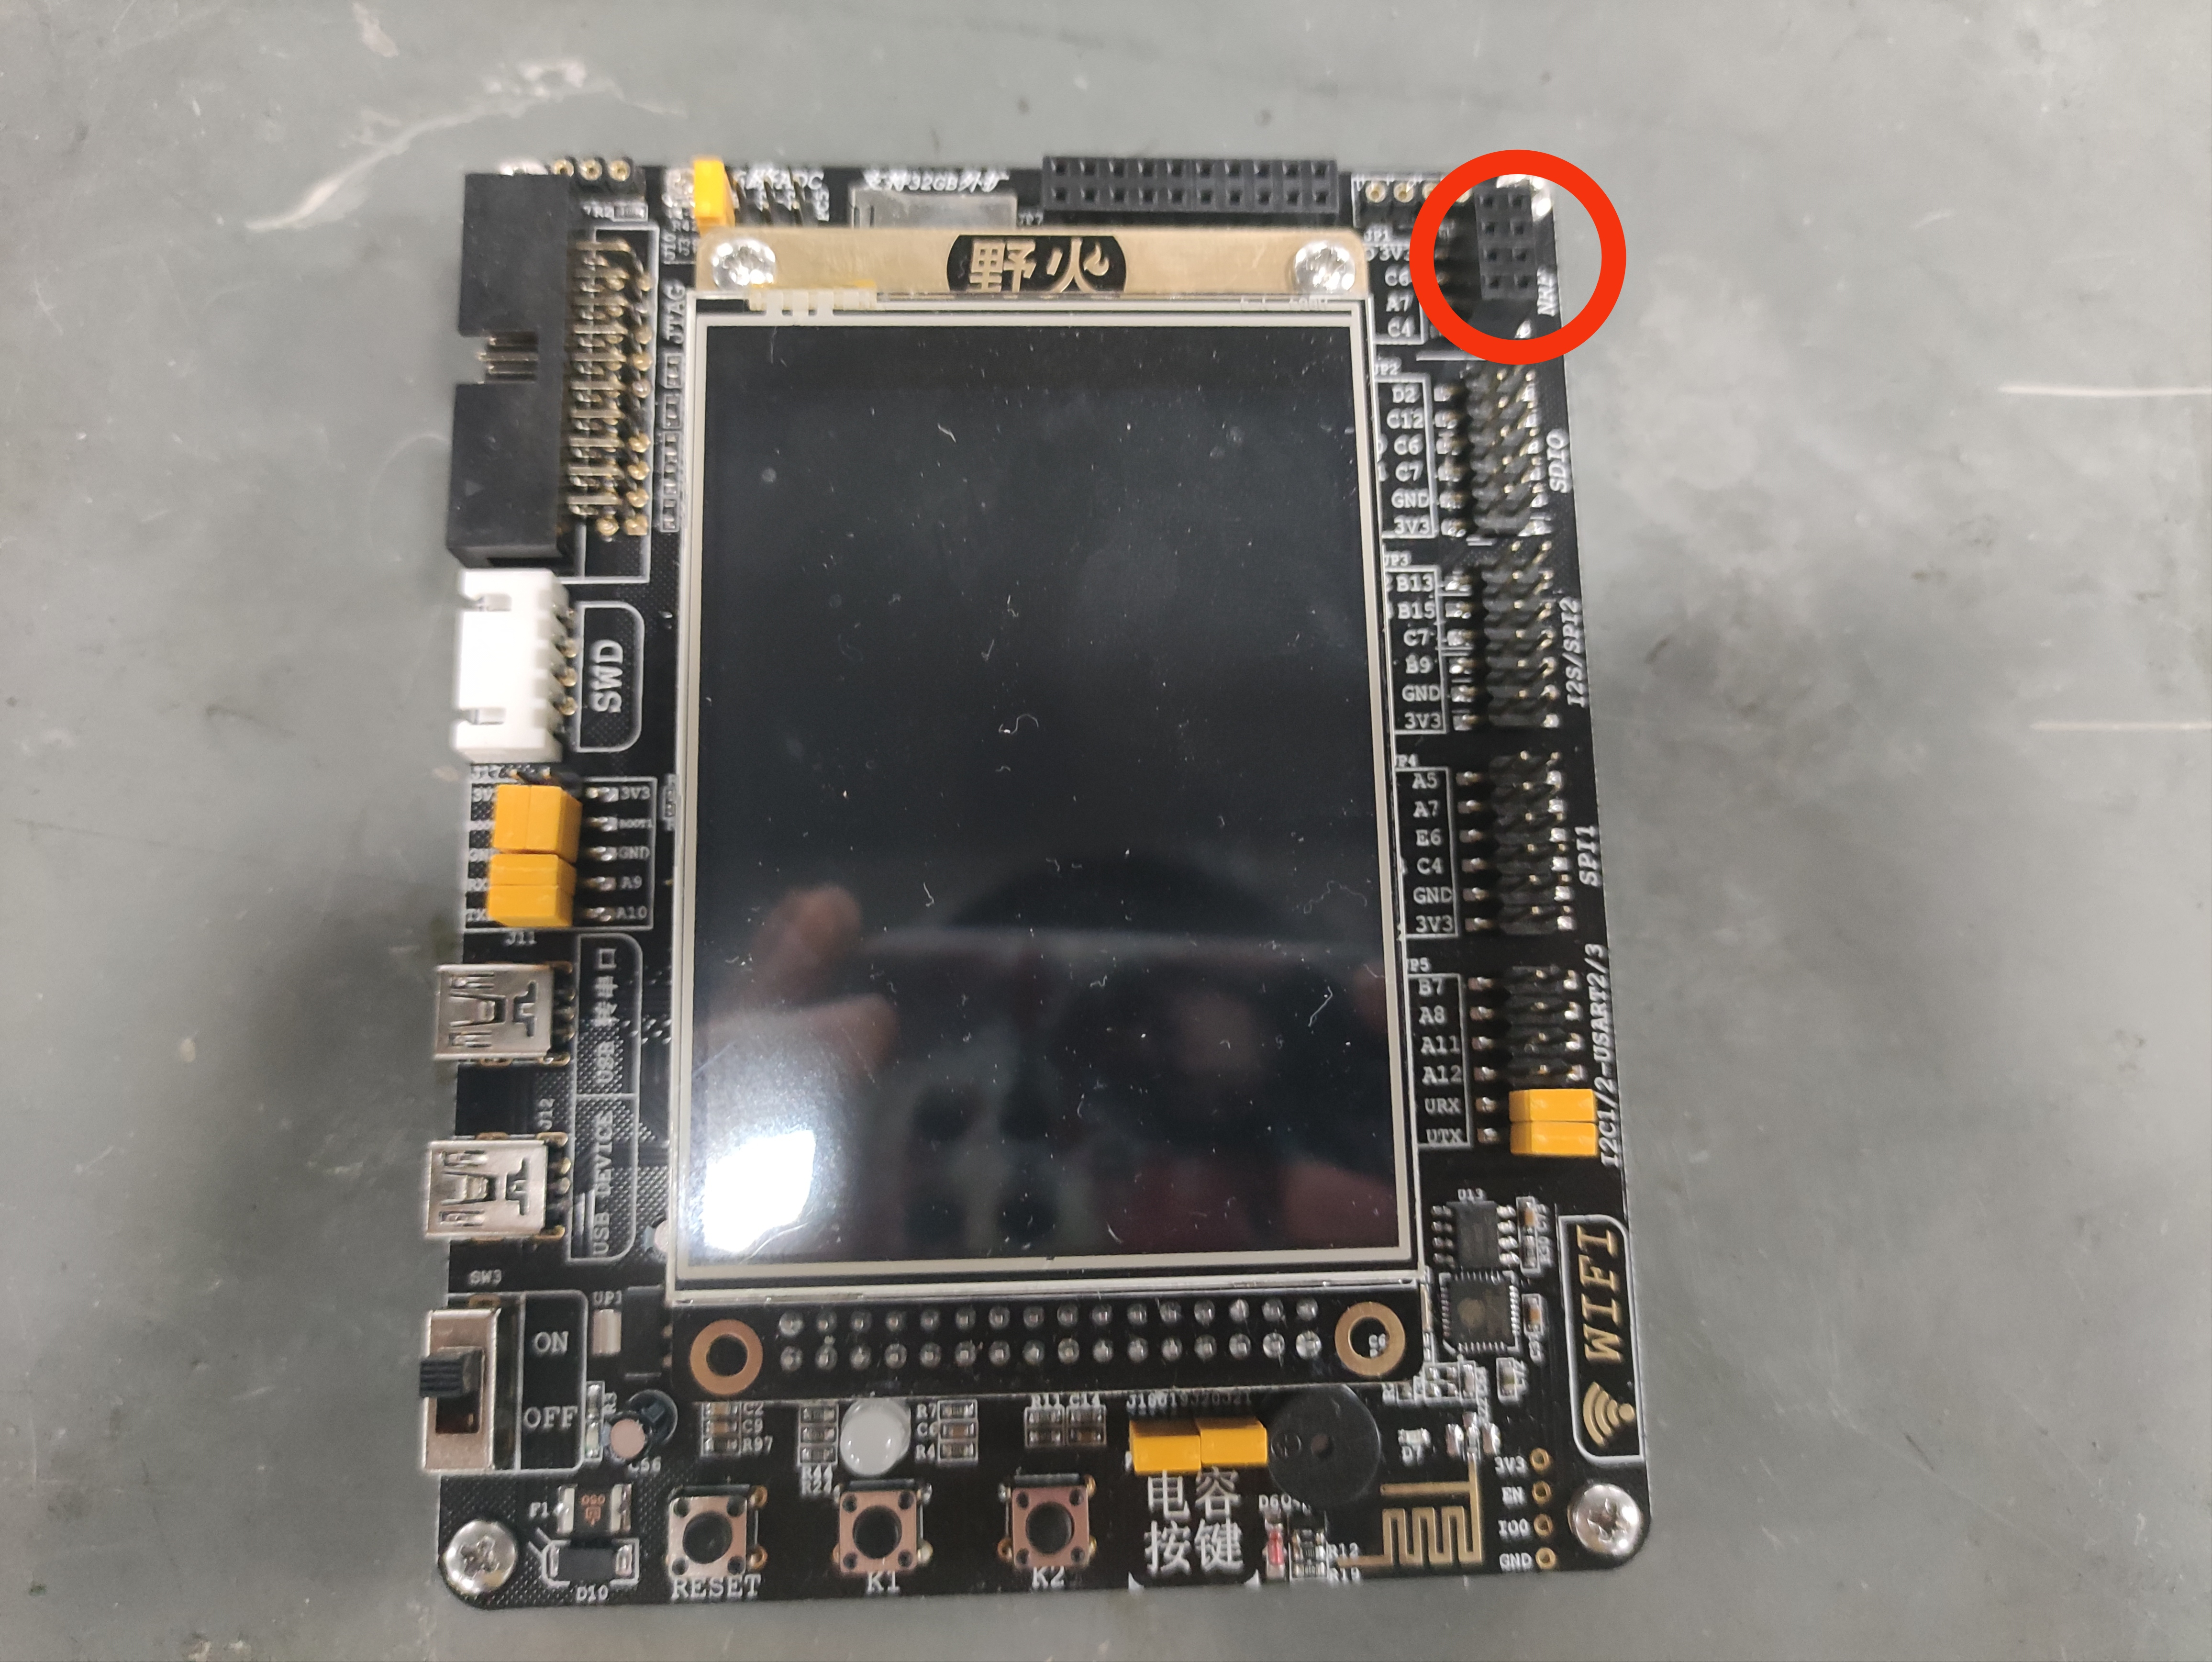
\includegraphics[scale=0.15]{p10.png}
\caption{坡印廷矢量}
\end{figure}

\textbf{坡印廷矢量}的定义为:
\begin{equation}
\overrightarrow{S}=\overrightarrow{E}\times\overrightarrow{H}
\end{equation}

其方向为能量流动的方向(如图10),单位为$W/m^2$。对于正弦电磁场,计算一个周期内的平均值更有意义。可以证明\textbf{平均坡印廷矢量}
\begin{equation}
\overrightarrow{S_{av}}=\frac{1}{2}Re[\overrightarrow{E}\times\overrightarrow{H}^*]
\end{equation}

由麦克斯韦方程组可以推出
\begin{equation}
\oint_S\overrightarrow{E}\times\overrightarrow{H}{\rm d}\overrightarrow{S}=\frac{\partial}{\partial t}\int\frac{1}{2}\mu_0H^2{\rm d}V+\frac{\partial}{\partial t}\int\frac{1}{2}\epsilon_0E^2{\rm d}V+\int\overrightarrow{E}\cdot\overrightarrow{J}{\rm d}V
\end{equation}

上式左边是单位时间进入闭合面$S$内部的电磁场能量,右边第一项是体积$V$内磁场能量的变化率,第二项是体积$V$内电场能量的变化率,第三项是焦耳热。该式被称为坡印廷定理。

\section{介质中的电磁场}
\subsection{介质极化和介质磁化}
为了简化模型,我们将物质分为导体和介质。

导体是一种含有大量可以自由移动的带电粒子的物质。自由移动的带电粒子可以是自由电子或带电离子。对应的导体分别是金属导体和电解质导体。金属导体比电解质导体的导电性强得多。

导体能够导电,是因为在导体内存在可自由移动的自由电子或带电离子。在金属导体内有可以任意移动的自由电荷,这些电荷做无规则热运动。如果无外力作用,整个导体呈中性。当导体周围上电场,电荷受到恒定外力时,自由电荷会发生定向移动,导体就会出现一端带正电一端带负电的现象。把导体中的电荷在外电场作用下发生重新分布的现象称为静电感应。导体上因感应而产生的电荷称为感应电荷。而“静电平衡”是指导体中的自由电荷所受的力达到平衡而不再做定向运动的状态,即导体内电场强度大小等于外加电场的电场强度,方向相反。

在静电场中导体具有如下性质:
\begin{itemize}
\item 导体内电场强度处处为零,否则导体内部的自由电子将在该电场的作用下继续运动,从而破坏导体静电平衡
\item 导体是一个等势体,表面是一个等势面,且电场强度与导体表面垂直
\item 导体内部净电荷为零,感应电荷只分布在导体表面上。否则导体内部同号电荷之间相互排斥而导致其向导体表面分散,直到内部净电荷为零
\end{itemize}

电介质实际上就是绝缘材料,其中不存在自由电荷。所谓磁介质,是指在外加磁场的作用下,能产生磁化现象,并能影响外磁场分布的物质。事实上,除了真空,其他任何物质都是可磁化的磁介质,只是磁化效应的强弱存在差别。

对于均匀电介质整体来说,在外电场作用下,垂直于电场的电介质的两个表面上出现正负电荷,然而这种电荷与导体中的自由电荷不同,它不能离开电介质,也不能在电介质内部自由移动,它们的移动范围会受到分子的约束,故称为束缚电荷(极化电荷)。

在外电场作用下,电介质中出现有序排列电偶极子以及表面上出现束缚电荷的现象,就提电介质的\textbf{极化}现象(如图11)。
\begin{figure}[htbp]
\centering
\includegraphics[scale=2]{p11.png}
\caption{极化现象}
\end{figure}

引入\textbf{极化强度}$\overrightarrow{P}$来描述电介质的极化特性或极化程度。定义为介质内部单位体积内所有电偶极矩矢量和(电偶极子和电偶极矩的分析,可参加教材p65)。可以证明:
\begin{equation}
\overrightarrow{D}=\epsilon_0\overrightarrow{E}+\overrightarrow{P}
\end{equation}

实验表明,线性各向同性均匀介质中的极化强度$\overrightarrow{P}$正比于外加电场$\overrightarrow{E}$,且与介质的电特性有关,即
\begin{equation}
\overrightarrow{P}=\epsilon_0\chi_e\overrightarrow{E}
\end{equation}

上式中的$\chi_e$是介质中的极化率,无量纲,是个常数。因此
\begin{equation}
\overrightarrow{D}=\epsilon_0(1+\chi_e)\overrightarrow{E}=\epsilon_0\epsilon_r\overrightarrow{E}=\epsilon\overrightarrow{E}
\end{equation}

上式中的$\epsilon_r$被称为\textbf{相对介电常数},常见材料的相对介电常数可参见教材p68。

利用极化强度可以求出束缚电荷面密度和体密度:
\begin{equation}
\begin{cases}
\rho_{PS}=\overrightarrow{P}\cdot\overrightarrow{e_n}\\
\rho_P=-\nabla\cdot\overrightarrow{P}\\
\end{cases}
\end{equation}

磁介质的分析和电介质类似(详细分析可参见教材p69),定义\textbf{磁化强度}$\overrightarrow{M}$表示介质内单位体积内磁偶极矩的矢量和,可以证明
\begin{equation}
\overrightarrow{B}=\mu_0(\overrightarrow{H}+\overrightarrow{M})=\mu_0(1+\chi_m)\overrightarrow{H}=\mu_0\mu_r\overrightarrow{H}=\mu\overrightarrow{H}
\end{equation}

上式中的$\mu_r$被称为\textbf{相对磁导率}。

利用磁化强度也可以求出束缚电流面密度和体密度:
\begin{equation}
\begin{cases}
\overrightarrow{J}_{MS}=\overrightarrow{M}\times\overrightarrow{e_n}\\
\overrightarrow{J}_M=\nabla\times\overrightarrow{P}\\
\end{cases}
\end{equation}

综上所述,如果我们要写出介质中的麦克斯韦方程组,其表现形式和式(67)是一样的,只是介质特性方程要改为:
\begin{equation}
\begin{cases}
\overrightarrow{B}=\mu\overrightarrow{H}\\
\overrightarrow{D}=\epsilon\overrightarrow{E}\\
\overrightarrow{J_c}=\sigma\overrightarrow{E}\\
\end{cases}
\end{equation}

\subsection{电磁场的边界条件}
在实际工作中,往往会涉及由不同的介质组成的电磁系统。从麦克斯韦方程组的微分形式和物态方程,只能获得一切电磁系统都适用的通解。若要获得给定电磁系统中的特解,还必须知道该系统中不同介质分界面的边界情况,以及电磁场在不同介质交界面上所遵循的规律——边界条件。

可以证明,电磁场5个场量的边界条件:
\begin{equation}
\begin{cases}
D_{1n}-D_{2n}=\rho_s\\
B_{1n}=B_{2n}\\
J_{1n}-J_{2n}=-\frac{\partial\rho_s}{\partial t}\\
E_{1s}=E_{2s}\\
H_{1s}-H_{2s}=J_s\\
\end{cases}
\end{equation}

对于两种理想介质的分界面(比如空气),其电导率为0。由$\overrightarrow{J}=\sigma\overrightarrow{E}$可知$J_s=0$,于是对于无源的理想介质分界面而言,有:
\begin{equation}
\begin{cases}
D_{1n}=D_{2n}\\
B_{1n}=B_{2n}\\
E_{1s}=E_{2s}\\
H_{1s}=H_{2s}\\
\end{cases}
\end{equation}

理想介质的电导率$\sigma=0$,而理想导体的电导率$\sigma=\infty$,工程上常将电导率很高的金属,如铜、铝、金、银等视为理想导体。在无源情况下,由于理想导体内部电场为零,根据麦克斯韦第一方程,其内部也不存在磁场。

因此在无源情况下,对于理想介质和理想导体分界面而言,其边界条件可简化为
\begin{equation}
\begin{cases}
D_n=\rho_s\\
B_n=0\\
E_s=0\\
H_s=J_s\\
\end{cases}
\end{equation}

上式表明:对于时变电磁场中的理想导体,电场总是与导体表面相垂直,而磁场总是与导体表面相切。导体内部既没有电场,也没有磁场。

\section{静态场的解}
在此之前,在分析电磁场问题时常常只考虑孤立带电体或孤立带电导线周围产生的电场与磁场,在讨论边界条件时,也只是讨论无限大的导体分界面或介质分界面的情况。但如果在电荷或带电体产生的场中放置一定形状的导体时,则该导体表面上将会产生感应电荷,这时源电荷和导体之间的区域内所产生的电场将是实际电荷与感应电荷所产生的电场的叠加。一般直接计算这种合成电场是比较复杂的,但是如果导体的形状较简单,而且源电荷又是点电荷或线电荷,则可以使用镜像法来计算它的合成场。

镜像法是利用一个称为镜像电荷的与源电荷相似的点电荷或线电荷来代替或等效实际电荷所产生的感应电荷,然后通过计算由源电荷和镜像电荷共同产生的合成电场,而得到源电荷与实际的感应电荷所产生的合成电场的方法。下面举两个例子。

设在真空中平面$xoy$为一导体,在$(0,0,h)$处有一电荷$q$,求电位分布(如图12)。
\begin{figure}[htbp]
\centering
\includegraphics[scale=0.3]{p12.png}
\caption{垂直镜面}
\end{figure}

可以证明,这个导体可以等效为在$(0,0,-h)$处有一电荷$-q$。

又因为在真空中,与电荷$q$距离为$r$的点电位为:
\begin{equation}
\phi=\frac{q}{4\pi\epsilon_0r}
\end{equation}

因此
\begin{equation}
\phi=\frac{q}{4\pi\epsilon_0}(\frac{1}{\sqrt{x^2+y^2+(z-h)^2}}-\frac{1}{\sqrt{x^2+y^2+(z+h)^2}})
\notag
\end{equation}

与上述结论类似,若导体以角的形式把一个点电荷围住,依然可以使用等效电荷求解(如图13)。
\begin{figure}[htbp]
\centering
\includegraphics[scale=0.3]{p13.png}
\caption{镜面法的推广}
\end{figure}
\begin{figure}[htbp]
\centering
\includegraphics[scale=0.5]{p14.png}
\caption{球形边界问题}
\end{figure}

另一个模型如图14,设接地导体球的半径为$a$,在球外与球心相距为$D$处有一点电荷$q$,计算球外的电位函数。

可以证明,在这种情况下,导体球可以等效为一个点电荷。这个点电荷$q'$在球心与原点电荷的连线上,与球心的距离为$d$,并且有
\begin{equation}
\begin{cases}
d=\frac{a^2}{d}\\
q'=-\frac{aq}{D}\\
\end{cases}
\end{equation}

如果导体球本身不接地,须在球心增加大小为$-q'$的等效电荷。

\section{理想介质中的均匀平面波}
\subsection{电磁波的波动方程}
在《大学物理》课程中,我们了解到往一个方向的波动满足一维波动方程,即
\begin{equation}
\frac{\partial^2\Psi}{\partial z^2}=\frac{1}{v^2}\cdot\frac{\partial^2\Psi}{\partial t^2}
\end{equation}

将此公式拓展到3维,即为
\begin{equation}
\nabla^2\Psi=\frac{1}{v^2}\cdot\frac{\partial^2\Psi}{\partial t^2}
\end{equation}

由麦克斯韦方程组的微分形式可以推出
\begin{equation}
\nabla^2\overrightarrow{E}=\mu\epsilon\cdot\frac{\partial^2\overrightarrow{E}}{\partial t^2}
\end{equation}
\begin{equation}
\nabla^2\overrightarrow{H}=\mu\epsilon\cdot\frac{\partial^2\overrightarrow{H}}{\partial t^2}
\end{equation}

由于在真空中,$c=\frac{1}{\sqrt{\mu_0\epsilon_0}}$,因此电磁场可以产生波动方程。式(92)(93)被称为\textbf{电磁波方程}。

对于时谐场而言,电磁波方程可以写成复数形式,即:
\begin{equation}
\nabla^2\overrightarrow{E}+k^2\overrightarrow{E}=0
\end{equation}
\begin{equation}
\nabla^2\overrightarrow{H}+k^2\overrightarrow{H}=0
\end{equation}

上式中,$k=\omega\sqrt{\mu\epsilon}$,被称为\textbf{相位常数}。

我们定义\textbf{均匀平面波}为电场强度值和磁场强度值在波阵面上处处相等的波。设在无限大的无源空间中,充满线性、各向同性的均匀理想介质,均匀平面波沿$z$轴传播,则有:
\begin{equation}
\frac{\partial\overrightarrow{E}}{\partial x}=\frac{\partial\overrightarrow{E}}{\partial y}=\frac{\partial\overrightarrow{H}}{\partial x}=\frac{\partial\overrightarrow{H}}{\partial y}=0
\end{equation}

故均匀电磁波的电场和磁场均无传播方向的分量,只有与传播方向垂直的分量。可以写出$\overrightarrow{E}$的表达式为:
\begin{equation}
\overrightarrow{E}(z,t)=\overrightarrow{e_x}E_1\cos(\omega t-kz+\phi_x)
\end{equation}

进而可以求得:
\begin{equation}
\overrightarrow{H}(z,t)=\overrightarrow{e_y}\sqrt{\frac{\epsilon}{\mu}}E_1\cos(\omega t-kz+\phi_x)
\end{equation}

从(97)(98)式可以看出,电场和磁场在空间上互相垂直坡印廷矢量的方向与波的传播方向一致。

\subsection{均匀平面波的传播特性}

由(97)(98)式可以看出,场量会随着$t$和$z$做周期性变化。$\omega t$和$kz$被分别称为\textbf{时间相位}和\textbf{空间相位}。由高中数学知识,\textbf{频率}$f$、\textbf{周期}$T$和\textbf{角频率}$\omega$的定义如下:
\begin{equation}
f=\frac{1}{T}=\frac{\omega}{2\pi}
\end{equation}

由《大学物理》的知识可知,\textbf{波长}$\lambda=vT$,又因为波速可以表示为$\frac{1}{\sqrt{\mu\epsilon}}$,因此有
\begin{equation}
\lambda=\frac{1}{f\sqrt{\mu\epsilon}}
\end{equation}

又因为相位常数$k=2\pi f\sqrt{\mu\epsilon}$,因此
\begin{equation}
k=\frac{2\pi}{\lambda}
\end{equation}

等相位面的移动速度被称为\textbf{相速度}:
\begin{equation}
v_p=\frac{\omega}{k}=\frac{1}{\sqrt{\mu\epsilon}}
\end{equation}

均匀平面波电场和磁场的振幅之比称为介质的波阻抗$\eta$,可以证明:
\begin{equation}
\eta=\sqrt{\frac{\mu}{\epsilon}}
\end{equation}

根据式(76),可以证明:
\begin{equation}
\overrightarrow{S_{av}}=\overrightarrow{e_z}\frac{1}{2\eta}E_{xm}^2
\end{equation}

\subsection{波的极化}
很明显,电磁波的电场强度肯定有不全在$x$轴的情况,当电场强度既有$x$方向的分量,又有$y$方向的分量时,电场强度可表示为:
\begin{equation}
\overrightarrow{E}(z,t)=\overrightarrow{e_x}E_1\cos(\omega t-kz+\phi_x)+\overrightarrow{e_y}E_2\cos(\omega t-kz+\phi_y)
\end{equation}

改写成复数形式则为:
\begin{equation}
\overrightarrow{E}(z)=(\overrightarrow{e_x}E_1e^{j\phi_x}+\overrightarrow{e_y}E_2e^{j\phi_y})e^{-jkz}
\end{equation}

因此相应的磁场强度为:
\begin{equation}
\overrightarrow{H}(z)=\frac{1}{\eta}\overrightarrow{e_z}\times\overrightarrow{E}(z)=(\overrightarrow{e_y}E_1e^{j\phi_x}-\overrightarrow{e_x}E_2e^{j\phi_y})e^{-jkz}
\end{equation}

为研究沿任意方向传播的均匀平面波,我们引入\textbf{波矢量}$\overrightarrow{k}$的概念,$\overrightarrow{k}$的模等于相位常数$k$,方向为均匀平面波的传播方向,所以有
\begin{equation}
\overrightarrow{k}=\overrightarrow{e_n}k=\overrightarrow{e_x}k_x+\overrightarrow{e_y}k_y+\overrightarrow{e_z}k_z
\end{equation}
\begin{equation}
\overrightarrow{E}=\overrightarrow{E_0}e^{-j(k_xx+k_yy+k_zz)}
\end{equation}

\begin{figure}[htbp]
\centering
\includegraphics[scale=0.3]{p15.png}
\caption{极化现象}
\end{figure}
若式(105)中电场强度两分量的相位不同步,那么就会产生波的\textbf{极化现象}。这种极化通常是用电场矢量$E$的尖端在空间随时间变化的轨迹来描述的。如果矢量的尖端在一条直线上运动,则称为线极化波。如果矢量尖端的运动轨迹是一个圆,则称为圆极化波。电场$E$的尖端的运动将描绘出一个椭圆,称为椭圆极化波。如果用右手的拇指指向波传播的方向,其他四指所指的方向正好与电场矢量运动的方向相同,则这个波就是右旋极化波,反之,称为左旋极化波。下面通过四个例子来解释。
\begin{equation}
\overrightarrow{E}=\overrightarrow{e_x}E_m\sin(\omega t-kz+\frac{\pi}{2})+\overrightarrow{e_y}E_m\cos(\omega t-kz)
\notag
\end{equation}

因为两分量相位相同,因此是线极化波。
\begin{equation}
\overrightarrow{E}=\overrightarrow{e_x}E_m\sin(\omega t-kz)+\overrightarrow{e_y}E_m\cos(\omega t-kz)
\notag
\end{equation}

因为$x$分量的波峰领先于$y$四分之一个周期且幅值相同,因此是左旋圆极化波。
\begin{equation}
\overrightarrow{E}=\overrightarrow{e_x}E_me^{-jkz}-\overrightarrow{e_y}je^{-jkz}
\notag
\end{equation}

因为$y$分量的波峰领先于$x$四分之一个周期且幅值相同,因此是右旋圆极化波。
\begin{equation}
\overrightarrow{E}=\overrightarrow{e_x}E_m\sin(\omega t-kz)+\overrightarrow{e_y}2E_m\cos(\omega t-kz)
\notag
\end{equation}

因为$x$分量的波峰领先于$y$四分之一个周期且幅值不同,因此是左旋椭圆极化波。

\section{有耗介质中的均匀平面波}
\subsection{有耗介质中的波动方程}
有耗介质也称为耗散介质,在这里是指电导率$\sigma\ne0$,但仍然保持均匀、线性及各向同性等特性。有耗介质中出现的传导电流会使在其中传播的电磁波发生能量损耗,从而导致波的幅值随着传播距离的增大而下降。研究表明,传播过程中幅值下降的同时,波的相位也会发生变化,致使整个传输波的形状发生畸变。

可以证明,在此情况下
\begin{equation}
\nabla\times\overrightarrow{H}=j\omega(\epsilon-j\frac{\sigma}{\omega})\overrightarrow{E}
\end{equation}

定义$\widetilde{\epsilon}$为有耗介质中的\textbf{等效复介电常数},则
\begin{equation}
\widetilde{\epsilon}=\epsilon-j\frac{\sigma}{\omega}
\end{equation}

因此,$\widetilde{k}^2=\omega^2\mu\widetilde{\epsilon}$,$\widetilde{k}=\omega\sqrt{\mu\widetilde{\epsilon}}$,$\widetilde{k}$被称为\textbf{复波数}。与上一章类似,我们依然可以用微分方程描述沿$z$轴方向传播的均匀平面波:
\begin{equation}
\nabla^2\overrightarrow{E}+\widetilde{k}^2\overrightarrow{E}=0
\end{equation}
\begin{equation}
\nabla^2\overrightarrow{H}+\widetilde{k}^2\overrightarrow{H}=0
\end{equation}

可以证明:
\begin{equation}
\overrightarrow{H}(z)=\frac{1}{\widetilde{\eta}}\overrightarrow{e_z}\times\overrightarrow{E}(z)
\end{equation}

式中,$\widetilde{\eta}=\sqrt{\frac{\mu}{\widetilde{\epsilon}}}$。

在有耗介质中,我们引入\textbf{传播常数}$\Gamma$:
\begin{equation}
\Gamma=j\widetilde{k}=\alpha+j\beta
\end{equation}

式中,$\alpha$为衰减常数,$\beta$为衰减常数。可以证明:
\begin{equation}
\widetilde{\eta}=\frac{\omega\mu}{\alpha^2+\beta^2}(\beta+j\alpha)
\end{equation}

因为$\alpha,\beta>0$,因此波阻抗成感性。若定义波阻抗的幅角$\theta={\rm arctan}\frac{\alpha}{\beta}$,波阻抗可以写成
\begin{equation}
\widetilde{\eta}=\frac{\omega\mu}{\sqrt{\alpha^2+\beta^2}}e^{j\theta}
\end{equation}

因为传导电流密度$\overrightarrow{J_c}=\sigma\overrightarrow{E}$,位移电流密度$\overrightarrow{J_d}=j\omega\overrightarrow{E}$,所以传导电流和位移电流幅值之比为$\frac{\sigma}{\omega\epsilon}$。由于传导电流会引起焦耳热损耗,因此可以将$\frac{\sigma}{\omega\epsilon}$作为反映介质相对损耗程度的因子。这个量被称为\textbf{损耗角正切},即
\begin{equation}
\tan\delta_c=\frac{\sigma}{\omega\epsilon}
\end{equation}

介质的相对损耗程度可以通过损耗角正切反映,可根据其取值范围的不同对不同介质进行如下分类:
\begin{itemize}
\item 理想介质,电导率$\sigma=0$,即传导电流为零,没有损耗
\item 良介质,$\frac{\sigma}{\omega\epsilon}\ll1$,即位移电流占绝对优势
\item 半导体,$\sigma$可与$\omega\epsilon$相比拟,即传导电流与位移电流具有相同数量级
\item 良导体:,$\frac{\sigma}{\omega\epsilon}\gg1$,即传导电流占绝对优势
\item 理想导体,$\sigma=\infty$,电磁波在理想导体中立刻衰减至零,说明在理想导体中没有场分布
\end{itemize}

需要指出的是, 同一种介质在不同频率下可能属于不同种类,因为介质的损耗角正切不仅取决于介质的电磁参数,还与工作频率密切相关。

\subsection{有耗介质中波的传播特性}
可以证明,在均匀、线性、各向同性的有耗介质中,沿$z$传播的均匀平面波的电磁场表达式为:
\begin{equation}
\overrightarrow{E}(z,t)=\overrightarrow{e_x}E_1e^{-\alpha z}\cos(\omega t-kz)
\end{equation}
\begin{equation}
\overrightarrow{H}(z,t)=\overrightarrow{e_y}\frac{E_1}{\lvert\widetilde{\eta}\rvert}e^{-\alpha z}\cos(\omega t-kz-\theta)
\end{equation}

在良介质中,由于$\frac{\sigma}{\omega\epsilon}\ll1$(一般取$\frac{\sigma}{\omega\epsilon}<0.01$),可以将各参数简化为:
\begin{equation}
\alpha\approx\frac{\sigma}{2}\sqrt{\frac{\mu}{\epsilon}}
\end{equation}
\begin{equation}
\beta\approx\omega\sqrt{\epsilon\mu}
\end{equation}
\begin{equation}
v_p=\frac{\omega}{\beta}\approx\frac{1}{\sqrt{\mu\epsilon}}
\end{equation}
\begin{equation}
\widetilde{\eta}\approx\sqrt{\frac{\mu}{\epsilon}}
\end{equation}

由此可得,良介质中波的传播有如下特点:
\begin{itemize}
\item 衰减常数不为0
\item $\beta$可以等效为上一章的$k$
\item 波阻抗近似为实数,电场和磁场近似为同相位,与理想情况类似
\end{itemize}

若电磁波在良导体中传播,可以证明:
\begin{equation}
\alpha=\beta\approx\sqrt{\pi f\mu\sigma}
\end{equation}
\begin{equation}
v_p=\frac{\omega}{\beta}\approx\sqrt{\frac{2\omega}{\mu\sigma}}
\end{equation}
\begin{equation}
\widetilde{\eta}=\sqrt{\frac{\pi f\mu}{\sigma}}(1+j)
\end{equation}

此时电磁波有以下特点:
\begin{itemize}
\item 衰减速度很快
\item 电磁波的相速度与频率有关
\item 波阻抗的相角$\theta=\frac{\pi}{4}$,磁场滞后电场八分之一周期的相位
\item 磁场能量远大于电场能量
\end{itemize}

\begin{figure}[htbp]
\centering
\includegraphics[scale=0.15]{p16.png}
\caption{趋肤效应}
\end{figure}

导电介质通常是作为导体使用的,但是,当交变电流通过导体时,电流密度在导体横截面上的分布是不均匀的,并且随着电流交变频率的升高,导体上所流过的电流将越来越集中于导体的表面附近,导体内部的电流越来越小,这种现象称为趋肤效应。(如图16)

为了对导电介质趋肤效应的程度进行定量表征,引入\textbf{趋肤深度}。将电磁波的振幅衰减到$e^{-1}$时它透入导电介质的深度定义为趋肤深度,用$\delta$表示。可以证明:
\begin{equation}
\delta=\frac{1}{\alpha}
\end{equation}

\subsection{群速和能速}
一个信号是由许多频率成分组成的,因此要确定一个信号在有耗介质中的传播速度很困难。这里引入\textbf{群速}的概念,它代表信号能量传播的速度。可以证明,群速
\begin{equation}
v_g=\frac{{\rm d}\omega}{{\rm d}k}
\end{equation}

对于相速与群速的关系,存在三种可能的情况:
\begin{itemize}
\item $\frac{{\rm d}v_p}{{\rm d}\omega}=0$,即相速与频率无关,$v_g=v_p$,表明不同波长的波速度相等,对应这种波所传播的介质应为无色散介质
\item $\frac{{\rm d}v_p}{{\rm d}\omega}<0$,即频率越高相速越小,$v_g<v_p$,表明波长大的波相速较大,对应这种波所传播的介质应为正常色散介质
\item $\frac{{\rm d}v_p}{{\rm d}\omega}>0$,即频率越高相速越大,$v_g>v_p$,表明波长大的波相速较小,对应这种波所传播的介质应为非正常色散介质
\end{itemize}

对于\textbf{能速},由于它表征波的能量的传播速度,而能量的流动情况可以由坡印廷矢量表示。在讨论能速的定义时,需要涉及电磁波的能量密度$\omega$,而其值在一个周期内的平均值更有实际意义。因此,能速的定义为
\begin{equation}
v_g=\frac{S_{av}}{\omega_{av}}
\end{equation}

可以证明,在无耗介质中,相速、群速和能速相等,都为$\frac{1}{\sqrt{\mu\epsilon}}$。在良导体中,$v_g=2v_p=2v_e\approx 2\sqrt{\frac{2\omega}{\mu\sigma}}$。

\section{波的反射与折射}
\subsection{垂直入射}
假设$xOy$是两介质的分界面,入射、反射和透射波分别是
\begin{equation}
\begin{cases}
\overrightarrow{E}_i(z)=\overrightarrow{e_x}E_{im}e^{-\Gamma_1 z}\\
\overrightarrow{H}_i(z)=\overrightarrow{e_y}\frac{E_{im}}{\widetilde{\eta}_1}e^{-\Gamma_1 z}\\
\end{cases}
\end{equation}

\begin{equation}
\begin{cases}
\overrightarrow{E}_r(z)=\overrightarrow{e_x}E_{rm}e^{\Gamma_1 z}\\
\overrightarrow{H}_r(z)=-\overrightarrow{e_y}\frac{E_{rm}}{\widetilde{\eta}_1}e^{\Gamma_1 z}\\
\end{cases}
\end{equation}

\begin{equation}
\begin{cases}
\overrightarrow{E}_t(z)=\overrightarrow{e_x}E_{tm}e^{-\Gamma_2 z}\\
\overrightarrow{H}_t(z)=\overrightarrow{e_y}\frac{E_{tm}}{\widetilde{\eta}_2}e^{-\Gamma_2 z}\\
\end{cases}
\end{equation}
定义分界面上的\textbf{反射系数}$R$为反射波电场的振幅与入射波电场振幅之比,\textbf{透射系数}$T$为折射波电场的振幅与入射波电场振幅之比,可得:
\begin{equation}
R=\frac{E_rm}{E_im}=\frac{\widetilde{\eta}_2-\widetilde{\eta}_1}{\widetilde{\eta}_2+\widetilde{\eta}_1}
\end{equation}
\begin{equation}
T=\frac{E_tm}{E_im}=\frac{2\widetilde{\eta}_2}{\widetilde{\eta}_2+\widetilde{\eta}_1}
\end{equation}

一般情况下, $R$和$T$是复数,表明在分界面上的反射和折射将引入一个附加租移。不难看出
\begin{equation}
R+1=T
\end{equation}

假设$xOy$是理想介质与理想导体的分界面,由于理想导体无内部电磁场,因此入射功率被全部反射。入射波和反射波表示如下:
\begin{equation}
\begin{cases}
\overrightarrow{E}_i(z)=\overrightarrow{e_x}E_{im}e^{-jk_1z}\\
\overrightarrow{H}_i(z)=\overrightarrow{e_y}\frac{E_{im}}{\eta_1}e^{-jk_1z}\\
\end{cases}
\end{equation}

\begin{equation}
\begin{cases}
\overrightarrow{E}_r(z)=-\overrightarrow{e_x}E_{im}e^{jk_1z}\\
\overrightarrow{H}_r(z)=\overrightarrow{e_y}\frac{E_{im}}{\eta_1}e^{jk_1z}\\
\end{cases}
\end{equation}

介质中合成波的表达式为:
\begin{equation}
\begin{cases}
\overrightarrow{E}_1(z,t)=\overrightarrow{e_x}2E_{im}\sin k_1z\sin\omega t\\
\overrightarrow{H}_1(z,t)=\overrightarrow{e_y}\frac{2E_{im}}{\eta_1}\cos k_1z\cos\omega t\\
\end{cases}
\end{equation}

由上式可知,合成电磁场形成驻波,电场和磁场之间有四分之一周期的相移,电场上的最大值点正好是磁场的最小值点。

可以证明,理想导体上的感应电流是:
\begin{equation}
\overrightarrow{J_s}=\overrightarrow{e_x}\frac{2E_{im}}{\eta_1}
\end{equation}

假设$xOy$是两理想介质的分界面,那么入射、反射和透射波符合式(131)(132)(133)。反射系数、入射系数和波阻抗都是实数,可以证明,合成电磁场有行波和驻波的叠加而成的\textbf{行驻波}。(可参见教材p177)

\subsection{斜入射}
\begin{figure}[htbp]
\centering
\includegraphics[scale=0.2]{p17.png}
\caption{斯涅尔定律}
\end{figure}

在《大学物理》中,几何光学有斯涅尔定律(如图17):
\begin{equation}
\theta_1=\theta_1^{'}\quad k_1\sin\theta_1=k_2\sin\theta_2
\end{equation}

假设$xOy$是两理想介质的分界面,在斜射条件下我们可以分为\textbf{垂直极化波}的斜入射和\textbf{平行极化波}的斜入射。垂直极化波即为入射波电场矢量的方向垂直于入射面$xOz$,所以入射波电场只有$y$方向的分量,可以证明(可参见教材p180):
\begin{equation}
R_n=\frac{\eta_2\cos\theta_i-\eta_1\cos\theta_t}{\eta_2\cos\theta_i+\eta_1\cos\theta_t}
\end{equation}
\begin{equation}
T_n=\frac{2\eta_2\cos\theta_i}{\eta_2\cos\theta_i+\eta_1\cos\theta_t}
\end{equation}

平行极化波即为入射波电场矢量的方向平行于入射面,因此入射波电场平行于$xOz$平面,可以证明(可参见教材p181):
\begin{equation}
R_s=\frac{-\eta_2\cos\theta_t+\eta_1\cos\theta_i}{\eta_2\cos\theta_t+\eta_1\cos\theta_i}
\end{equation}
\begin{equation}
T_s=\frac{2\eta_2\cos\theta_i}{\eta_2\cos\theta_t+\eta_1\cos\theta_i}
\end{equation}

当电磁波以某一入射角入射到两种介质分界面上时,如果反射系数为0,则全部电磁能量都进入到第二种介质,这种情况称为\textbf{全折射}。出现全折射时对应的入射角就是\textbf{布儒斯特角},用$\theta_B$表示。

可以证明,垂直极化波不可能出现全折射。对于一般的非磁性介质,平行极化波的布儒斯特角为
\begin{equation}
\theta_B={\rm arctan}\sqrt{\frac{\epsilon_2}{\epsilon_1}}
\end{equation}

当电磁波入射到两种介质分界面上时,如果反射系数$\lvert R\rvert=1$,则投射到分界面上的电磁波将全部反射回第种介质中,这种情况称为\textbf{全反射}。可以证明,电磁波从光密介质入射到光疏介质时,若入射角大于\textbf{临界角},则发生全反射,入射角表示为:
\begin{equation}
\theta_c={\rm arcsin}\frac{k_2}{k_1}
\end{equation}
\end{document}